Having identified the various activities needed to be done, we agreed on the milestones for the project, which can be found in Appendix \ref{app:milestones}.
In the planning of how to reach these milestones we focused on dependencies
between activities (e.g. the design of the web service API needed to be done before the
web service could be produced).

To map out dependencies, we used a dependency diagram (which can be found in Appendix
\ref{app:dependencydiagram}: a network diagram using the activity on-node format\cite[ch.~8.5]{caye}.
In this version of the network diagram, each box (node) represents an activity with
dependencies represented as arrows between them. The method uses the concepts of
\textbf{earliest start time}/\textbf{earliest finish time} and \textbf{latest start
time}/\textbf{latest finish time} in addition to the activity’s own estimated duration.

\begin{figure}[hbtp]
   \centering
    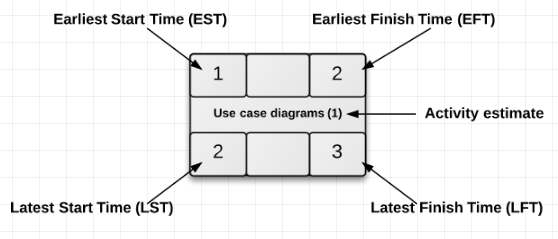
\includegraphics[scale=0.5]{./Empiri/Planning/img/networkdiagramnotation.png}
    \caption{The layout of a node in the dependency diagram with its data explained. These nodes are connected with arrows, to signify dependence.}
\end{figure}
 
The EST/EFT can be found by a \emph{forward pass} through the diagram, while the LST/LFTs
can be found by a following \emph{backward pass}. These numbers leave us with the
\emph{critical path}, which consists of those activities that, if delayed, would delay
the whole project (in other words, those that must keep the deadline).

It also gives a clear presentation of the \emph{total slack} (how much an activity can
be postponed), \emph{free slack} (how much an activity can be postponed without affecting
following activities), and \emph{head slack} (how much an activity can be postponed without
delaying the whole project deadline) for each activity.